\documentclass[10pt]{article}
\usepackage[a4paper,total={6in,8in}]{geometry}
%\usepackage{a4wide}
\usepackage{comment}
\usepackage{graphicx}
\usepackage{esint}    			 %package for integrals%
%\usepackage[utf8]{inputenc}
%\usepackage{attachfile}
\usepackage{layout}
%\usepackage{wrapfig}
\usepackage{listings}
\usepackage{url}
\usepackage{color}


%\graphicspath{ {/home/putlurhitheshreddy/Desktop/} }


\begin{document}
	
\begin{center}
	\textbf{\Large Assignment-8}\\
	\vspace{1mm}
	\textbf{\Large ELP-718 Telecom Software Laboratory}\\
	\textbf{Putlur Hithesh Reddy} \\
	\textbf{2018JTM2244} \\
	\textbf{2018-2020 }\\ 
	\textbf{A report presented for the assignment on \textbf{Python and github}} \\ [1.5 in]	
\end{center}

\begin{figure}[h!]
	\centering
	
\includegraphics{iitlogo} \\  [1.5 in]	
\end{figure}

\begin{center}
	\textbf{Bharti School of}\\ 
\textbf{Telecommunication Technology and Management }\\
\textbf{IIT DELHI}\\
\textbf{India}\\
\textbf{27-Sep-2018}
\end{center}

\newpage
\tableofcontents
\newpage

\section{\textbf{\Large Objective}}
 The assignment is designed to know about Python and the ease of programming in python. This also introduces to the basic usage of github and its relevance in software development life cycle
 
 
 
 
\section{\textbf{\large Problem Statement-1}}
\subsection{Problem Statement}
\textbf{Finding Valid Cross}
\begin{itemize}
		\item IIT Delhi, has just got the strongest computer
		\item The professors in charge wants to check the computational capacity of the computer
		\item So, they decided to create the problem which is to be given as an assignment to students​
		\item You have to help the professor to check the computation capability of the computer
		\item A valid cross is defined here as the two regions (horizontal and vertical) of equal lengths crossing over each other
		\item These lengths must be odd, and the middle cell of its horizontal region must cross the middle cell of its vertical region
		\item Find the two largest valid crosses that can be drawn on smart cells in the grid, and return two integers denoting the dimension of the each of the two largest valid crosses
		\item In the above diagrams, our largest crosses have dimension of 1,  5 and 9 respectively 
		\item The two crosses cannot overlap, and the dimensions of each of the valid crosses should be maximal
\end{itemize}

\subsection{Algorithm and implementation}

\begin{itemize}
		\item n and m are taken from the user and checked for the given constraint
		\item \cite{1} Strings are taken form the user into a list
		\item Each string is taken and started from each element and searched for S
		\item Valid crosses are defined in functions
		\item Each element of the matrix is sent to the functiona nd checked for valid cross
\end{itemize}

\newpage

%\subsection{Flow-chart}
%\begin{figure}[h!]
%	\centering
%	\includegraphics[scale=0.6]{Screenshot3}
%\end{figure}

\subsection{constraints}
\begin{itemize}
	\item n lies between 2 and 105
	\item m lies between 2 and 105
\end{itemize}

\subsection{Input and Output Format}
\begin{itemize}
		\item \textit{Input Format}
		\subitem The first line contains two space-separated integers,  n and m
		\subitem Each of the next  lines n contains a string of  m characters where each character is either S (Smart) or D (Dull)		
		\subitem These strings represent the rows of the grid
		\subitem If the jth character in the ith  line is S, then  (i,j) is a  cell smart
		\subitem Otherwise it's a  dull cell
		\item \textit{Output Format}
		\subitem \cite{2}
		\subitem Find two valid crosses that can be drawn on smart cell of the grid, and return the dimension of both the crosses in the reverse sorted order(i.e. First Dimension should be the larger one and other should be smaller one)
\end{itemize}

\subsection{Test cases or Sample Inputs and Respective results}
\begin{itemize}
		\item \textit{Sample Input 0}
		\item 5 6 
		\item SSSSSS
		\item SDDDSD
		\item SSSSSS
		\item SSDDSD
		\item SSSSSS
		
		\item \textit{Sample output 0}
		\item 5 1
		
		\item \textit{Sample Input 1}
		\item 6 6 
		\item DSDDSD
		\item SSSSSS
		\item DSDDSD
		\item SSSSSS
		\item DSDDSD
		\item DSDDSD
		
		\item \textit{Sample output 0}
		\item 5 5 there can be more than one valid crosses of the same dimension, you can consider any
		
		\item \textit{Sample Input 2}
		\item 5 9 
		\item SSSSDSDDD
		\item DDSDDDDDD
		\item SSSSSDDDD
		\item DDSDDSDDD
		\item DSSSDDDDD
		
		\item \textit{Sample output 0}
		\item 9 1
\end{itemize}

\subsection{Difficulties faced}
\begin{itemize}
	\item Deciding the functions to be used
	\item Comparing cell blocks with starting element or middle element
\end{itemize}

\newpage





\section{\textbf{\large Problem Statement-2}}
\subsection{Problem Statement}
\textbf{Finding encrypted messades }
\begin{itemize}
		\item After, getting mix results of valid crosses, professors decided to test the computation abilities on one more problem
		\item This time professors wanted to test the decryption capabilities of the computer
		\item Encryption of  a message requires three keys, k1, k2, and k3
		\item The 26 letters of English and underscore are divided in three groups,  [a-i] form one group, [j-r] a second group, and everything else ([s-z] and underscore) the third group
		\item Within each group the letters are rotated left by ki positions in the message
		\item Each group is rotated independently of the other two. Decrypting the message means doing a right rotation by ki positions within each group	
\end{itemize}

\subsection{Algorithm and implementation}
\begin{itemize}
		\item All the required inputs are taken from the user
		\item The inputs are checked for constraints
		\item Groups given are considered as lists
		\item Empty lists are defined and element sare stored into them after grouping
		\item \cite{3}The obtained list are rotated and the respective decrypted message is printed onto the console
\end{itemize}

\newpage

%\subsection{Flow-chart}
%\begin{figure}[h]
%	\centering
%	\includegraphics[scale=0.5]{Screenshot2}
%\end{figure}
\subsection{constraints}
\begin{itemize}
	\item Length of the string lies between 1 and 150
	\item ki lies between 1 and 150 (i=1,2,3)
\end{itemize}

\subsection{Input and Output Format}
\begin{itemize}
	\item \textit{Input Format}
	\subitem All input strings comprises of only lowercase English alphabets and underscores
	\item \textit{Output Format}
	\subitem For each encrypted message, the output is a single line containing the decrypted string 
\end{itemize}

\subsection{Test cases or Sample Inputs and Respective results}
\begin{itemize}
	\item \textit{Sample Input 1}
	\subitem 2 3 4
	\subitem dikhtkor\_ey\_tec\_ocsusrsw\_ehas\_
	
	\item \textit{Sample Output 1}
	\subitem hardwork\_is\_the\_key\_to\_success
\end{itemize}

\subsection{Difficulties faced}
\begin{itemize}
	\item String to list conversion
	\item Rotating the list
\end{itemize}

\newpage

\section{\textbf{\large C Programming Codes}}
\lstinputlisting{ps1.py}
\lstinputlisting{ps2.py}
%\begin{verbatim}
%\end{verbatim}

\section{\textbf{\large Screenshots related to coding}}
\begin{figure}[h!]
	\centering
	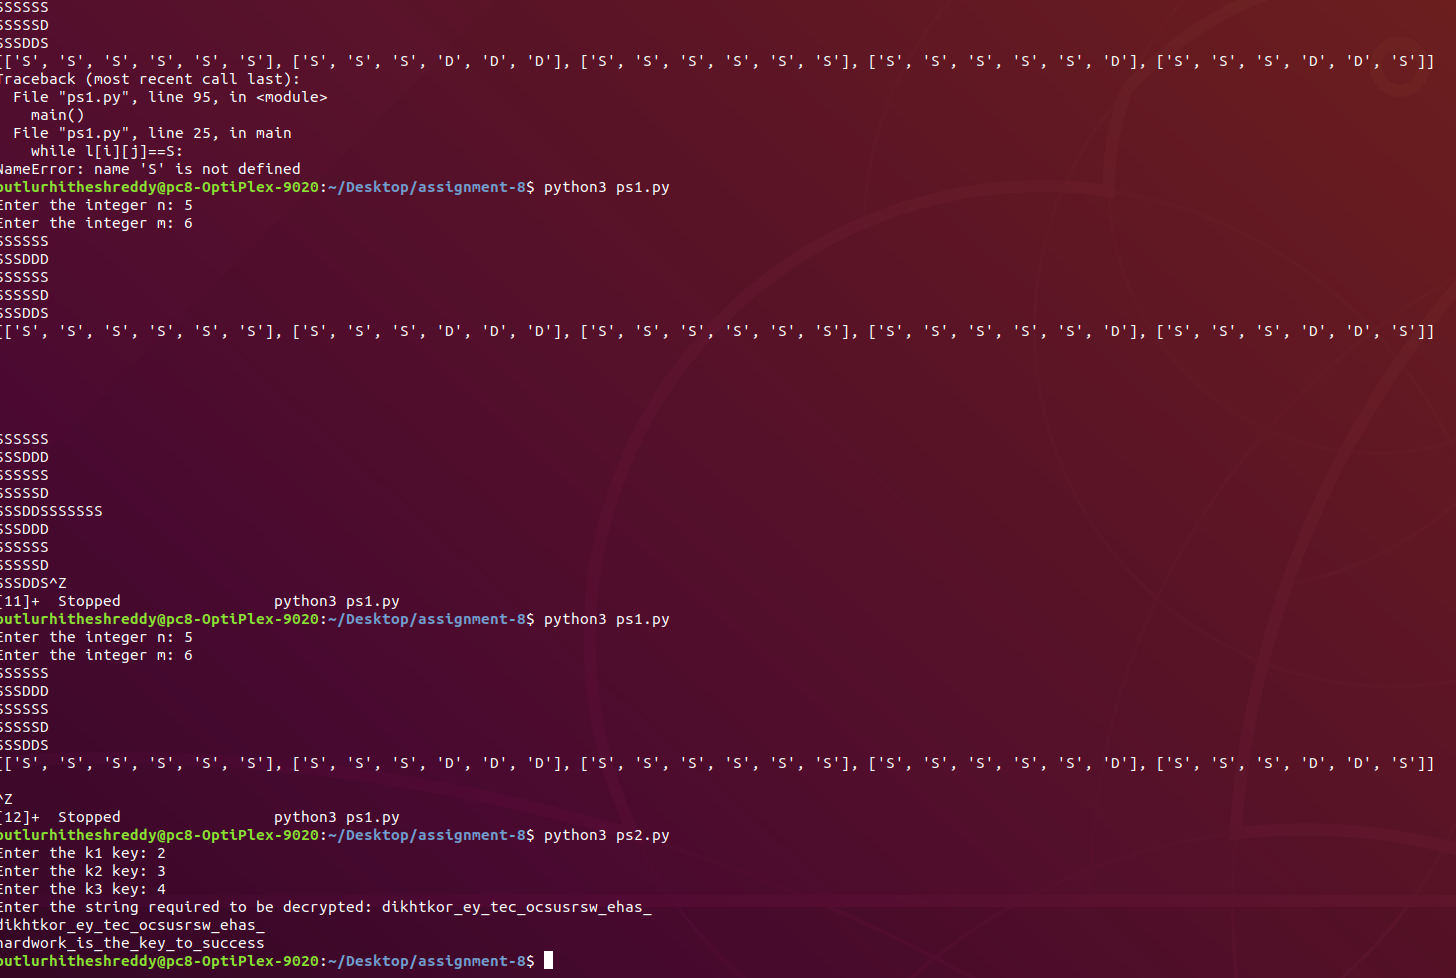
\includegraphics[width=15cm,height=8.5cm]{Screenshot1}
\end{figure}
%\begin{figure}
%	\centering
%	\includegraphics[width=15cm,height=15cm]{Screenshot2}
%\end{figure}
%\begin{figure}
%	\centering
%	\includegraphics{Screenshot3}
%\end{figure}

\newpage

\bibliographystyle{plain} \bibliography{citations.bib}

\end{document}